\chapter{Описание алгоритма}
\label{cha:ch_2}

В данной главе будет описано обратимое и устойчивое к искажениям преобразование для построения спектрограммы из аудиосигнала.
Оно строится на основе операции многоканальной 1D свертки с заранее сформированным ядром, а также некоторой постобработки.

\section{Теоретическое обоснование алгоритма}
Напомним формулу 1D свертки. Пусть на входе есть двумерный массив данных $x: [L_{in} \times  C_{in}]$ 
и ядро свертки в виде массива $K: [C_{out} \times N \times C_{in}]$. Также задан шаг свертки $s$.
Тогда результат операции $y: [L_{out} \times C_{out}]$ рассчитывается по следующей формуле:
\begin{equation}
	y[i, c_{out}] = \sum_{j=0}^{N-1} \sum_{c_{in}=0}^{C_{in}-1} x[i \cdot s + j, c_{in}] \cdot K[c_{out}, j, c_{in}]
\end{equation}
\[i \in [0, L_{out}), \quad c_{out} \in [0, C_{out})\]
\[L_{out} = \lfloor(L_{in} - N) / s\rfloor + 1\]

\begin{figure}
  \centering
  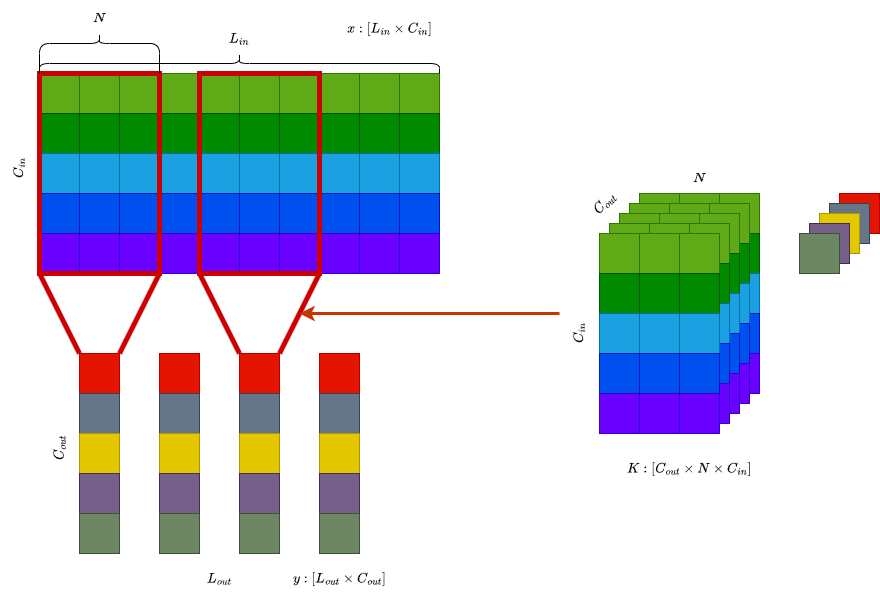
\includegraphics[width=0.9\linewidth]{figures/conv1d_drawio}
  \caption{Иллюстрации операции 1D свертки}
  \label{fig:conv1d_drawio}
\end{figure}

Каждый вектор $y_i: [1 \times C_{out}]$ можно рассматривать как матричное умножение вырезанного окна $x_i: [1 \times (N \cdot C_{in})]$ на матрицу $K^T: [(N \cdot C_{in}) \times C_{out}]$.

В случае, когда входным массивом является аудиосигнал, количество входных каналов $C_{in} = 1$, и можно несколько упростить формулу. 
\[x: [L_{in}], \quad K: [C_{out} \times N]\]
\begin{equation}
	y[i, c_{out}] = \sum_{j=0}^{N-1} x[i \cdot s + j] \cdot K[c_{out}, j]
\end{equation}


\textbf{Дискретное оконное преобразование Фурье (STFT)} можно посчитать через 1D свертку, если сформировать ядро $K_{\mathrm{stft}}: [N \times N]$ следующим образом:
\begin{equation}
	K_{\mathrm{stft}}[k, n] = e^{-i\pi \frac{(n - N/2) \cdot k}{N}} * w[n]
\end{equation}

\textbf{Дискретное вейвлет-преобразование (DWT)} на основе вейвлета Морле можно построить с помощью свертки с таким ядром:
\begin{equation}
	K_{\mathrm{dwt}}[k, n] = \psi^* \left(\frac{n - N/2}{a_0^k}\right)
\end{equation}
\[\psi(t) = e^{i\pi t} * e^{-\left(\frac{\pi t}{2\sigma}\right)^2}, \quad   a_0 \in (1, \infty)\]

На рисунке \ref{fig:stft_kernel} изображены ядра сверток для указанных преобразований, а также для преобразования, которое будет описано в данной работе.

\begin{figure}
  \centering
  \subfigure{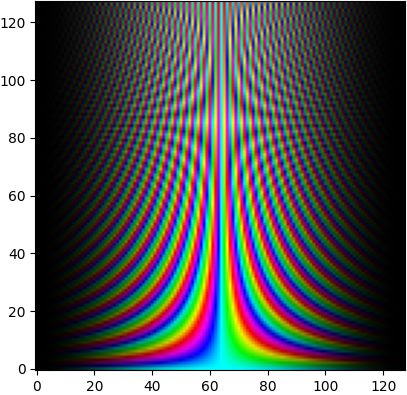
\includegraphics[width=0.3\textwidth]{figures/stft_kernel}} 
  \subfigure{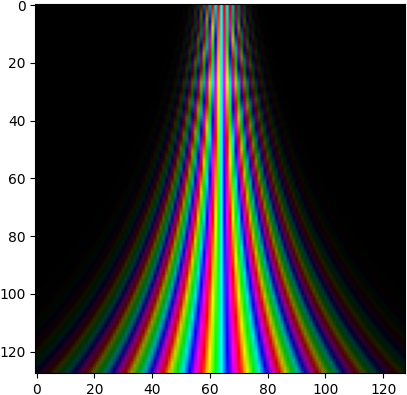
\includegraphics[width=0.3\textwidth]{figures/dwt_kernel}} 
  \subfigure{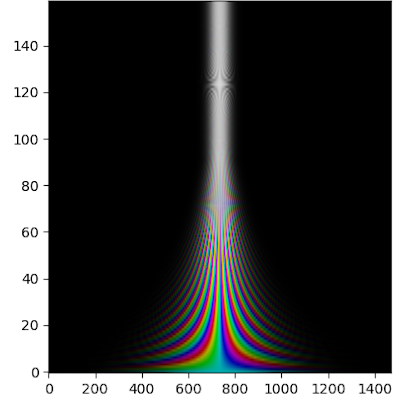
\includegraphics[width=0.3\textwidth]{figures/my_kernel}} 
  \caption{Ядро 1D свертки для STFT (1), вейвлет преобразования (2) и предлагаемого в работе преобразования (3)}
  \label{fig:stft_kernel}
\end{figure}


Теперь опишем процесс восстановления сигнала с помощью свертки, и при каких условиях он возможен.

Для начала рассмотрим преобразование, дискретное по частотам, но непрерывное по времени, 
представляющее собой свертку сигнала $x(t)$ с вейвлетом $\psi_m(t) = \Delta f_m \cdot e^{2\pi i f_m t} \cdot w(t\,\Delta f_m)$.
Здесь $\Delta f_m$ - расстояние между соседними частотами на выбранной шкале частот. $w(t)$ - оконная функция, она должна быть симметричной.

\begin{equation}
  S_m(t)=\int \limits _{-\infty}^{+\infty}x(\tau)\,\psi_m(t - \tau)\,d\tau = \{x * \psi_m\}(t)
  \label{eq:conv_x_psi}
\end{equation}

Здесь и далее, запись $\{u*v\}(t)$ обозначает свертку в математическом смысле, которая определяется следующим образом:

\begin{equation}
  \{u*v\}(t)\triangleq \int \limits_{-\infty }^{\infty }u(\tau )v(t-\tau )\,d\tau = \int \limits_{-\infty }^{\infty }u(t-\tau )v(\tau )\,d\tau
\end{equation}

Полученная в равенстве \ref{eq:conv_x_psi} функция $S_m(t)$ представляет собой сигнал, ограниченный некоторой полосой частот, 
определяемой центральной частотой $f_m$ и спектральной шириной окна $\Delta f_m$.
Если посчитать спектр сигнала $S_m(t)$ с помощью преобразования Фурье, то, согласно теореме о свертке \cite{conv_theorem}, 
получим произведение спектра исходного сигнала $\mathcal{F}\{x(t)\}$ и спектра вейвлета $\mathcal{F}\{\psi_m(t)\}$.
Спектр вейвлета представляет собой спектр оконной функции, центр которого сдвинут к частоте $f_m$.

\begin{equation}
  \mathcal{F}\{S_m\}(f) = \mathcal{F}\{x\}(f) \cdot \mathcal{F}\{\psi_m\}(f)
\end{equation}

Если произвести снова свертку $S_m(t)$ с вейвлетом $\psi_m(t)$ в качестве этапа восстановления и посчитать спектр полученного сигнала, получим:

\begin{equation}
  \tilde{x}_m(t) = \{S_m * \psi_m\}(t) = \int \limits _{-\infty}^{+\infty} S_m(\tau)\,\psi_m(t - \tau)\,d\tau
\end{equation}
\begin{equation}
  \mathcal{F}\{\tilde{x}_m\} = \mathcal{F}\{S_m\} \cdot \mathcal{F}\{\psi_m\} = \mathcal{F}\{x\} \cdot (\mathcal{F}\{\psi_m\})^2
\end{equation}

Заметим, что спектр вейвлета является действительным в силу его симметричности $\psi(-t) = \psi^{*}(t)$, и равен спектру оконной функции, сдвинутым к центральной частоте $f_m$:
\begin{equation}
  \mathcal{F}\{\psi_m\}(f) = \Delta f_m \cdot \mathcal{F}\{w(t\,\Delta f_m)\}(f - f_m) = \mathcal{F}\{w(t)\}\left(\frac{f - f_m}{\Delta f_m}\right)
\end{equation}

При достаточно плотном перекрытии окон на оси частот, спектр исходного сигнала $\mathcal{F}\{x\}$ можно представить как взвешенную сумму:
\begin{equation}
  \mathcal{F}\{x\} = \frac{
    \sum \limits_m \mathcal{F}\{x\} \cdot (\mathcal{F}\{\psi_m\})^2
  }{
    \sum \limits_m (\mathcal{F}\{\psi_m\})^2
  } = 
  \frac{
    \sum \limits_m \mathcal{F}\{\tilde{x}_m\}(f)
  }{
    \sum \limits_m (\mathcal{F}\{\psi_m\})^2(f)
  }
  \label{eq:back_weighted_sum}
\end{equation}

Если записать спектр каждого вейвлета как сдвинутый и растянутый спектр окна, получим следующее равенство:

\begin{equation}
  \mathcal{F}\{x\} = 
  \frac{
    \sum \limits_m \mathcal{F}\{\tilde{x}_m\}(f)
  }{
    \sum \limits_m (\mathcal{F}\{w(t)\})^2 \left(\frac{f - f_m}{\Delta f_m}\right)
  }
  \label{eq:wavelets_back_spec}
\end{equation}


Для получения обратной формулы покажем, что при достаточно плотном перекрытии окон на оси частот
знаменатель последней дроби является константой на любой частоте $f$ и рассчитаем его.

\textbf{Утверждение 1}. Рассмотрим сумму в знаменателе как интеграл по частотам.
Если ввести функцию шкалы частот $f(m)$ и рассмотреть рассточние между частотами $\Delta f_m$ как производную этой функции $\frac{df}{dm}$,
данная сумма будет стремиться к интергалу следующего вида, который равен $w(0)$:
\begin{equation}
\sum \limits_m \mathcal{F}\{w(t)\} \left(\frac{f_0 - f_m}{\Delta f_m}\right) 
  \xrightarrow[M \to \infty]{} 
\int \limits_{-\infty}^\infty \mathcal{F}\{w(t)\} \left(\frac{f_0 - f(m)}{\frac{df}{dm}}\right) \, dm
  = I
\end{equation}
\[
I = w(0) + \varepsilon
\]

\textbf{Доказательство} для значения интеграла:

Разложив $f(m)$ по формуле Тейлора до первой производной, получим:
\begin{equation}
  f_0 - f(m) = (m_0 - m) \cdot \frac{df}{dm} + \frac{1}{2} \frac{d^2f(\theta)}{dm^2} (m - m_0)^2
\end{equation}

Если в пределах ширины окна функция $f(m)$ почти линейна, последний член пренебрежимо мал по сравнению с первым. 
Всегда можно отмасштабировать оконную функцию так, чтобы на каждой частоте в пределах ширины окна функция $f(m)$ была почти линейной, 
и вклад нелинейности в значение интеграла был бы меньше требуемого числа $\varepsilon$. Отметим, что на практике используется сумма, 
а не интеграл, и незначительная ошибка все равно возникает.

Потставляя полученное разложение в равенство для интеграла $I$, получим следующее выражение:
\begin{equation}
  I = 
  \int \limits_{-\infty}^\infty \mathcal{F}\{w(t)\} \left(\frac{(m_0 - m) \cdot \frac{df}{dm}}{\frac{df}{dm}}\right) \, dm = 
  \int \limits_{-\infty}^\infty \mathcal{F}\{w(t)\} \left(m_0 - m\right) \, dm
\end{equation}

Поскольку спектр оконной функции симметричен, можно заменить переменную в интеграле с $m_0 - m$ на $m$, 
и тогда по одному из свойств преобразования Фурье, интеграл по всему спектру $\mathcal{F}\{w(t)\}$ будет равен значению прообраза в нуле $w(0)$.

\begin{equation}
  I = 
  \int \limits_{-\infty}^\infty e^{2\pi i 0 m} \mathcal{F}\{w(t)\} (m) \, dm = w(0)
\end{equation}

В итоге получаем, что 
\begin{equation}
  \sum \limits_m \mathcal{F}\{w(t)\} \left(\frac{f_0 - f_m}{\Delta f_m}\right)  \cong  w(0)
\end{equation}

В формуле для спектра восстановленного сигнала в знаменателе стоит сумма \textit{квадратов} спектров окон:
\begin{equation}
  K_{\psi} = \sum \limits_m (\mathcal{F}\{w(t)\})^2 \left(\frac{f - f_m}{\Delta f_m}\right) = \mathcal{F}^{-1}\{\mathcal{F}\{w(t)\}^2\}(0)
\end{equation}

По теореме о свертке
\begin{equation}
  K_{\psi} = \{w * w\}(0) = \int \limits_{-\infty}^\infty w^2(t) \, dt
\end{equation}

В итоге, подставляя сумму $K_{\psi}$ в формулу \ref{eq:back_weighted_sum}, в силу линейности преобразования Фурье, 
получим такую формулу для обратного преобразования:
\begin{equation}
  x(t) = \frac{1}{K_{\psi}} \, \sum \limits_m \tilde{x}_m(t) = \frac{1}{K_{\psi}} \, \sum \limits_m \{S_m * \psi_m\}(t)
\end{equation}

Отметим, что данная формула справедлива даже когда вейвлеты и ширина их окон не упорядочены по правилу $\psi_m = \psi(\frac{t}{a_0^m})$, 
но вместо этого ширина окон должна быть пропорциональна расстоянию между соседними частотами $\Delta f_m$.

Теперь соберем вместе формулы прямого и обратного преобразования вместе с вспомогательными функциями и константами:

\begin{equation}
  \psi_m(t) = \Delta f_m \cdot e^{2\pi i f_m t} \cdot w(t\,\Delta f_m)
\end{equation}
\begin{equation}
  \Delta f_m = (f_{m+1} - f_{m-1}) / 2
\end{equation}

Формула прямого преобразования через свертку:
\begin{equation}
  S_m(t) = \{x * \psi_m\}(t)
\end{equation}

Формула обратного преобразования через свертку:
\begin{equation}
  x(t) = \frac{1}{K_{\psi}} \, \sum \limits_m \{S_m * \psi_m\}(t)
  \label{eq:back_conv_x_kpsi}
\end{equation}
\begin{equation}
  K_{\psi} = \int \limits_{-\infty}^\infty w^2(t) \, dt
\end{equation}

Набор значений $f_m$ должен покрывать весь спектр исходного сигнала. Функция $f(m)$ должна быть почти линейной на каждом отрезке $m \pm 1$.
В случае, если сигнал действительный, можно оставить только положительные частоты и умножить правую часть равенства \ref{eq:back_conv_x_kpsi} на 2.
Также напомним, что оконная функция $w(t)$ должна быть симметричной и обеспачивать локализацию сигнала во временной и в частотной области.

На практике операция свертки производится над дискретизированным сигналом. Вместо интеграла используется сумма, 
а окно смещается по времени с определенным шагом $\Delta t$:
\begin{equation}
  \{u*v\}[n] = 
  \sum \limits_{ k = -K }^{ K } u( k\,\delta t ) \, v( n\,\Delta t - k\,\delta t ) \, \delta t = 
  \sum \limits_{ k = -K }^{ K } u( n\,\Delta t - k\,\delta t ) \, v( k\,\delta t ) \, \delta t
\end{equation}

В таком случае для восстановимости сигнала шаг свертки должен быть меньше минимальной ширины окна: 
$ \Delta t \, \lesssim \, \min \limits_m (1/\Delta f_m) $


\subsection{Выбор оптимальной шкалы частот}

Описанное преобразование позволяет строить спектрограмму и восстанавливать звук сразу в выбранной шкале частот. 
В отличие от спектрограммы, построенной при помощи STFT, 
ее не нужно переводить из линейной шкалы в другую, теряя часть информации. 

Остается определить, какая шкала частот лучше всего подойдет для построения спектрограммы 
в качестве промежуточного представления звука в задачах синтеза речи.

Большинство нейросетей для распознавания и синтеза речи, которые работают со спектрограммами, используют мел-шкалу из-за того, что она отражает
разрешающую способность человеческого слуха в частотной области. Ее вполне можно использовать как основу для данного преобразования.

Однако, есть одна особенность, на которую стоит обратить внимание: 
для полной восстановимости шаг свертки должен быть меньше минимальной ширины окна. 
Если использовать логарифмическую или мел-шкалу, но при этом не соблюдать условие $ \Delta t \, \lesssim \, \min \limits_m (1/\Delta f_m) $,
тогда в области высоких частот, где оно начинает нарушаться и между окнами возникают зазоры, сигнал восстанавливается неточно, 
и могут возникать артефакты в виде дополнительных шумов. Человеческий слух не отличает одну реализацию шума от другого, 
поэтому в некоторых случаях можно не выполнять это условие в области высоких частот.
На рисунке \ref{fig:spec_diff} изображены спектрограммы до и после восстановления, и их разность в случае, 
когда условие, ограничивающее шаг свертки не выполняется. На последнем рисунке видно, 
что разность теряется в шумах и может быть не различима человеком.

\begin{figure}[t]
  \centering
  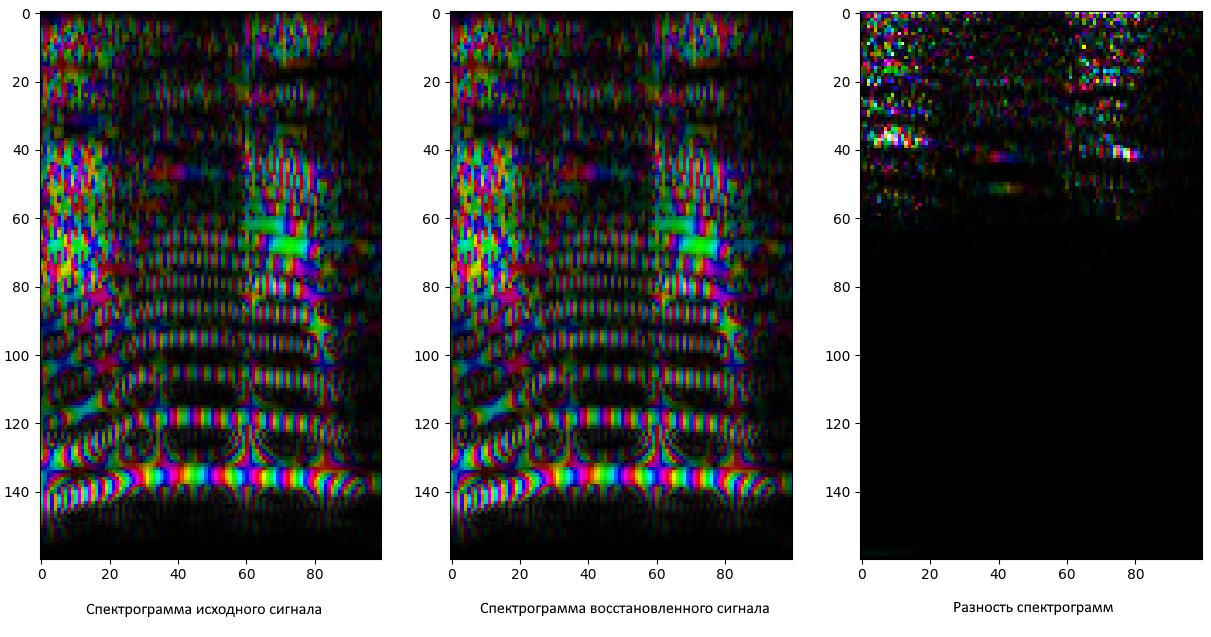
\includegraphics[width=0.8\linewidth]{figures/spec_diff}
  \caption{Спектрограмма сигнала до и после восстановления и их разность}
  \label{fig:spec_diff}
\end{figure}

В случае когда требуется восстановить сигнал максимально точно, необходимо будет выбрать очень маленький шаг свертки.
Маленький шаг свертки ведет к большому количеству точек и большому размеру массива, получаемого в результате преобразования. 
При выборе нелинейной шкалы размеры окон по времени на низких частотах обычно больше шага свертки, что приводит к 
повторению похожих значений в соседних по времени точках, и как следствие к избыточности информации. 
С одной стороны, это повышает устойчивость обратного преобразования к точечным искажениям, 
но с другой стороны приводит к большему потреблению вычислительных ресурсов. 
Иными словами, спектрограмма в нелинейной шкале содержит избыточность информации из-за большего наложения окон в области низких частот.

Если взять за основу мел-шкалу $f(m)$ и ограничить сверху ее производную $df/dm$, 
то в области высоких частот функция $f(m)$ будет переходить из экспоненциальной в линейную, и 
расстояние между соседними частотами $\Delta f_m < \Delta f_{max}$ будет ограничено сверху, 
и можно будет выбрать соответствующий шаг свертки $\Delta t \, \lesssim \, 1 / \Delta f_{max}$. 
Он будет больше, чем для мел-шкалы, что позволит сократить размеры выходного массива, 
при этом сохранив удобную шкалу в области низких и средних частот. 
Если в практическом приложении можно пожертвовать небольшим растяжением области высоких частот, где обычно расположены шумы и шипящие согласные,
то можно использовать такую комбинированную шкалу, чтобы сократить размеры по времени, сохранив восстановимость сигнала.
Пример спектрограммы сигнала до и после восстановления в такой комбинированной шкале и их разность приведены на рисунке \ref{fig:spec_diff_combo_scale}

\begin{figure}
  \centering
  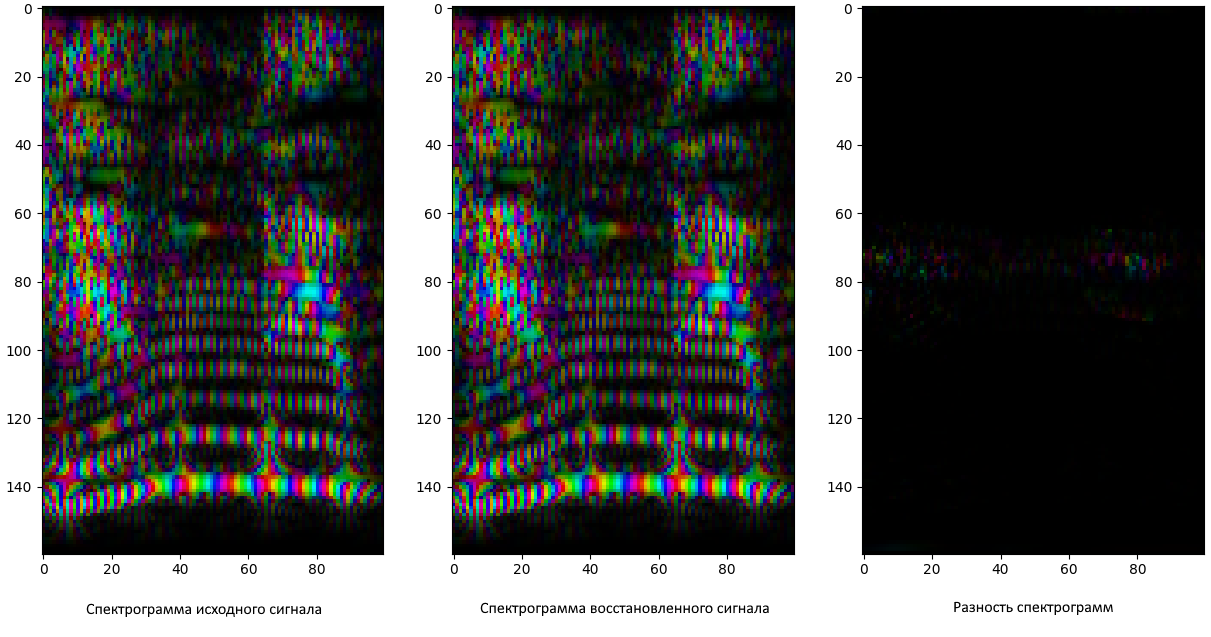
\includegraphics[width=0.8\linewidth]{figures/spec_diff_combo_scale}
  \caption{Спектрограмма сигнала до и после восстановления в комбинированной шкале частот и их разность}
  \label{fig:spec_diff_combo_scale}
\end{figure}







\begin{markdown}
 - избыточность информации в шумах
 - представление с сохранением фазы
 - представление с производной фазы
 - представление с магнитудой
 - Алгоритм Гриффина-Лима
  - адаптация
  - более точное восстановление при сохранении фазы
 - картинки
\end{markdown}

\section{Реализация алгоритма}
\begin{markdown}
 - описание алгоритма
   - подготовка ядра
     - шкала частот, df
	 - окна для каждой частоты
	 - Фурье базис с окнами, нормировка
	 - маска наложений
	 - ядро прямого прохода
	 - ядро обратного прохода
   - прямое преобразование
     - свертка
	 - преобразование фазы
	   - либо ничего
	   - либо производная фазы
	   - либо только магнитуда
	 - шкала амплитуд
   - обратное преобразование
     - шкала амплитуд
	 - восстановление фазы
	   - либо ничего
	   - либо интеграл (при этом накапливаются ошибки)
	   - либо GriffinLim
	 - свертка
 - масштабирование
 - восстановление шумов
 - рекомендуемые значения параметров
 - код на Python
 - предложения для быстрой реализации
 - ускорение на GPU и TPU
 - визуализация спектрограмм
\end{markdown}

\section{Выводы по главе}
